\section{Infraestrutura}

\subsection{Arquitetura}

Em seguida é apresentada a arquitetura da infraestrutura escolhida.

--- IMAGEM

\subsection{Storage}
Esta componente é responsável por garantir alta disponibilidade e lidar com a persistência, quer nas máquinas, quer nos discos que a compõem. Tendo em conta o dito anteriormente optou-se por colocar dois discos para persistência de dados do website, e outros dois discos para armazenar a base de dados PostgreSQL. Para lidar com cada par de discos despenderam-se duas máquinas que contem os serviços DRBD e iSCSI. O primeiro serviço simula dois RAID1, onde a caracteristica é a replicação de dados, que no futuro, além da disponibilidade em caso de falha, torna-se bastante útil nas laeituras de disco. O segundo serviço é responsavel por permitir o acesso estes discos remotamente, através de TCP/IP, que usufrui do armazenamento de dados que o serviço anterior oferece.

\subsection{Cluster}
O Service Cluter é uma componente essencial nesta infraestrutura devido à garantia que fornece quanto à alta disponibilidade. Este Cluster é composto por dois serviços, o PostgreSQL e NFS Server garantindo assim a disponibilidade inicialmente em duas máquinas e em caso de alguma falhar, então os serviçoes vão correr em apenas uma das máquinas, o que certamente irá reduzir o nivel de desempenho, mas sem nunca perder o serviço, visto que se pode agir quando o cluster manager informar que tal aconteciemento se sucedeu.

\subsection{WEB}
Esta componente apenas vai receber e atender os pedidos que chegam do exterior, ou seja, contêm o serviço httpd para interpretar os pedidos e o NFS Cliente, que se conecta ao NFS Server do Cluster, onde terá acesso aos ficheiros que necessita para a interpretação e resposta do pedido.
O projeto Graphite é um sistema de gráficos em tempo real altamente escalável. Os dados podem ser visualizados através de interfaces web do Graphite.

\subsection{LVS}
Para garantir que a infraestrutura é estável e segura, foi necessário usar algo que fizesse a distribuição de carga pelos servidores da componente Web. Tendo isto em conta, foi decidido incluir duas máquinas com serviços responsáveis por saberem para onde enviar os pedidos. Para além da distribuição de carga que estes servidores conseguem efetuar, protegem ainda a infraestrutura do mundo exterior, nomeadamente através de Virtual IP, por onde os clientes acedem ao serviço que a infraestrutura dispõe. Desta forma os servidores funcionam tambem como uma Firewall, onde são filtrados os pedidos que não são esperados pela infraestrutura, atribuindo assim, a segurança falada.
O balanceador de carga fica entre o utlziador e os servidores Web Apache de back-end que mantêm o mesmo conteúdo. Se um deles está em baixo, todos os pedidos serão automaticamente redirecionados para o servidor backend restante. o que significa que os utilizadores não notarão qualquer interrupção do serviço.

\subsection{Configurações}

\subsection{Storage}
-----------
MUDAR IPS AQUI 
-----------

Para a configuração da nossa Storage precisamos de dois ingredientes, duas máquinas virtuais, sendo uma cliente e outra servidor, e acesso ao Cluster criado.
Primeiramente no servidor devem ser executados os seguintes comandos:
\framebox[1.1\width]{yum install scsi-target-utils} \par
\framebox[1.1\width]{cat /etc/tgt/targets.conf} \par
    <target iqn.2010-04.nl.meinit:node1.target1>
    backing-store /iscsi1.img
    initiator-address 172.16.0.2
    </target>
\framebox[1.1\width]{dd if=/dev/zero of=/iscsi1.img bs=1024 count=102400} \par
\framebox[1.1\width]{chkconfig tgtd on} \par
\framebox[1.1\width]{service tgtd start} \par

De seguida, em todos clientes devem ser inseridos os seguintes comandos:
\framebox[1.1\width]{yum install iscsi-initiator-utils} \par
\framebox[1.1\width]{service iscsi start} \par
\framebox[1.1\width]{iscsiadm -m discovery -t sendtargets -p 172.16.0.1} \par
\framebox[1.1\width]{iscsiadm -m node -T iqn.2010-04.nl.meinit:node1.target1 -p 172.16.0.1 -l} \par
\framebox[1.1\width]{chkconfig iscsi on} \par

Finalmente, e para concluir a configuração, é necessário criar e montar o filesystem no cliente:
\framebox[1.1\width]{fdisk /dev/sda} \par
\framebox[1.1\width]{mkfs.ext3 /dev/sda1} \par
%\framebox[1.1\width]{echo "/dev/sda1 /mnt ext3 defaults,_netdev 0 0\" >>  /etc/fstab} \par


\subsection{Cluster}

\subsection{WEB}

\subsection{LVS}
O pretendido é ter um balanceador de carga, onde a máquina irá analisar todos os servidores web definindo qual estará disponivel para dar resposta ao pedido efetuado.
A infraestrutura for pensada de forma redundante para que no caso de falha de um deles, o outro possa continuar a interpretar os pedidos, e sendo assim os utilizadores obtêm sempre uma resposta aos seus pedidos.
Para a configuração do LVS foram instalados 3 serviços, o HAProxy que será usado como software de balanceamento de carga, o Keepalived que será usado como solução de alta disponibilidade e o Apache que será utilizado como software para carga de equilíbrio. Em seguida são apresentados os comandos necessários para a configuração destes serviços.


HAProxy

Nos servidores haproxy1 e haproxy2, devemos primeiramente instalar o pacote do HAProxy:
\framebox[1.1\width]{yum install -y haproxy} \par

Em seguida abrir o ficheiro \verb+/etc/haproxy/haproxy.cfg+ usando um editor de texto, e substituir a linha \verb+frontend  main \*:5000+ por \verb+frontend  main *:8+ e comentar a linha \verb+use_backend static if url_static+.
Proseguindo para o final do ficheiro, devem ser retiradas as linhas que começam com “server app” e adicionadas as seguintes linhas:
\framebox[1.1\width]{server httpd1 192.168.0.103:80 check} \par
\framebox[1.1\width]{server httpd2 192.168.0.104:80 check} \par

De seguida, ativar o boot e iniciar o serviço HAProxy:
\framebox[1.1\width]{server httpd2 192.168.0.104:80 check} \par
\framebox[1.1\width]{systemctl enable haproxy} \par
\framebox[1.1\width]{systemctl start haproxy} \par

Abrindo agora o ficheiro /etc/firewalld/services/haproxy.xml, devem ser colocadas as seguintes linhas:
<?xml version="1.0" encoding="utf-8"?>
<service>
<short>HAProxy</short>
<description>HAProxy load-balancer</description>
<port protocol="tcp" port="80"/>
</service>

No próximo passo é necessário corrigir o contexto do SELinux e permissões do ficheiro haproxy.xml:
\framebox[1.1\width]{cd /etc/firewalld/services} \par
\framebox[1.1\width]{restorecon haproxy.xml} \par
\framebox[1.1\width]{chmod 640 haproxy.xml} \par

Finalmente deve-se fazer update da configuração da firewall:
\framebox[1.1\width]{firewall-cmd --permanent --add-service=haproxy} \par
\framebox[1.1\width]{firewall-cmd --reload} \par

Keepalived

Para instalar o pacote do keepalived:
\framebox[1.1\width]{yum install -y keepalived} \par

De seguida é necessário criar um novo arquivo /etc/keepalived/keepalived.conf com as seguintes linhas de código:

\begin{figure}[!h]
\begin{MyVerbatim}
vrrp_script chk_haproxy {
  script "killall -0 haproxy" # check the haproxy process
  interval 2 # every 2 seconds
  weight 2 # add 2 points if OK
}

vrrp_instance VI_1 {
  interface eth0 # interface to monitor
  state MASTER # MASTER on haproxy1, BACKUP on haproxy2
  virtual_router_id 51
  priority 101 # 101 on haproxy1, 100 on haproxy2
  virtual_ipaddress {
    192.168.0.100 # virtual ip address 
  }
  track_script {
    chk_haproxy
  }
}
\end{MyVerbatim}
\end{figure}


De seguida, para ativar o serviço keepalived na inicialização do sistema é necessário correr os seguintes comandos:
\framebox[1.1\width]{systemctl enable keepalived} \par
\framebox[1.1\width]{systemctl start keepalived} \par

Finalmente é preciso verificar a presença do VIP no servidor haproxy1:


\begin{figure}[!h]
\begin{MyVerbatim}
# ip a

1: lo: <LOOPBACK,UP,LOWER_UP> mtu 65536 qdisc noqueue state UNKNOWN
link/loopback 00:00:00:00:00:00 brd 00:00:00:00:00:00
inet 127.0.0.1/8 scope host lo
valid_lft forever preferred_lft forever
inet6 ::1/128 scope host
valid_lft forever preferred_lft forever
2: eth0: <BROADCAST,MULTICAST,UP,LOWER_UP> mtu 1500 qdisc pfifo_fast state UP qlen 1000
link/ether 52:54:00:f7:2a:a9 brd ff:ff:ff:ff:ff:ff
inet 192.168.0.101/24 brd 192.168.0.255 scope global eth0
valid_lft forever preferred_lft forever
inet 192.168.0.100/32 scope global eth0
valid_lft forever preferred_lft forever
inet6 fe80::5054:ff:fef7:2aa9/64 scope link
valid_lft forever preferred_lft forever
\end{MyVerbatim}
\end{figure}

Apache

Para a instalação do Apache é necessário a criação de um ficheiro index.html em /var/www/html do httpd1 e colocar o seguinte comando:
\framebox[1.1\width]{Test httpd1} \par

Como passo seguinte, é necessário fazer o mesmo para o servidor httpd2, mas substituir por httpd2 no ficheiro index.html:
\framebox[1.1\width]{Test httpd2} \par

Para testar a configuração através de outro servidor basta utilizar os seguintes comandos:
\framebox[1.1\width]{yum install -y elinks} \par
\framebox[1.1\width]{elinks http://192.168.0.100} \par

\subsection{Ambiente de Testes}

-- Não sei se é assim ou não
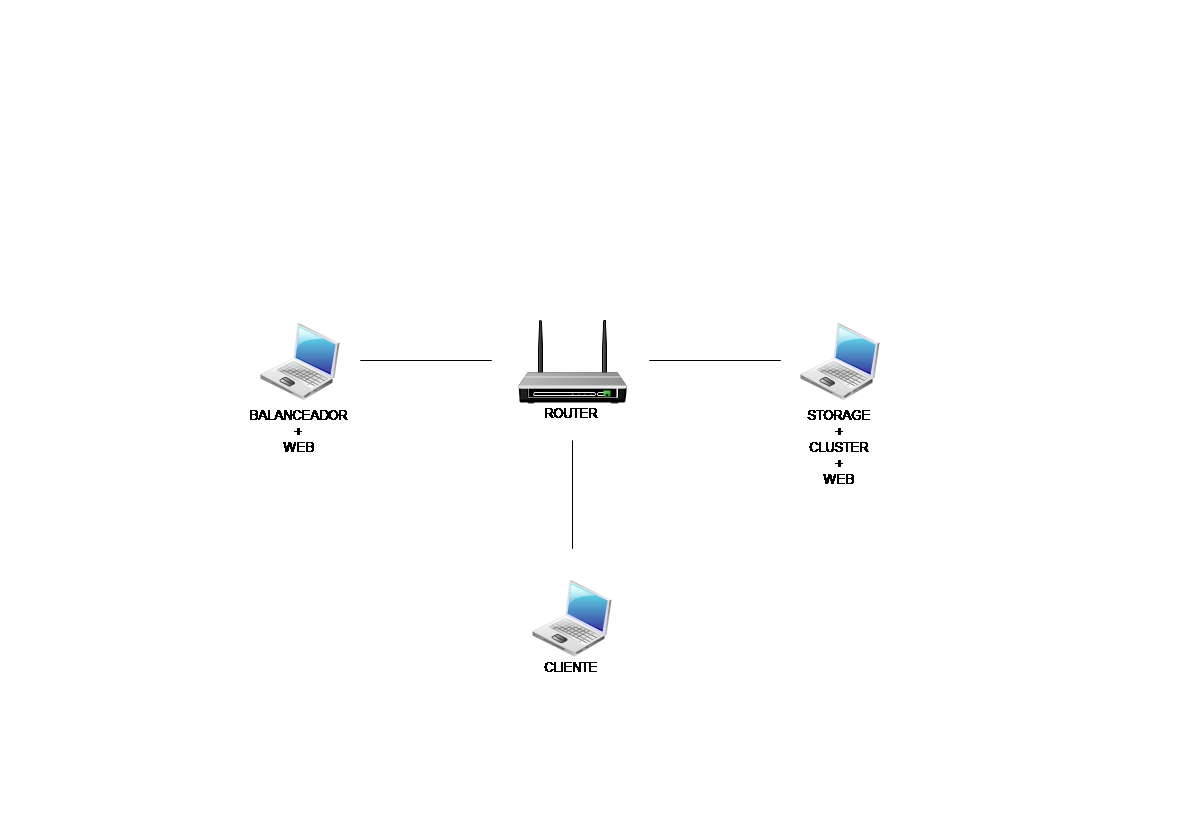
\includegraphics[scale=.4]{img/AmbienteDeTestes}

\subsection{Testes realizados e análise}

